\documentclass{beamer}
\usepackage{pgfpages}
%\setbeameroption{show notes on second screen=left} %enable for notes
\usepackage{graphicx}
\usepackage{xcolor}
\usepackage{listings}
\usepackage{hyperref}
\lstset{language=python,frame=single}
\usepackage{verbatim}
\usepackage{subcaption}
\usepackage{amsmath}
\usepackage{relsize}
\usepackage{appendixnumberbeamer}
\usepackage{xparse}
\usepackage{multimedia}
\usepackage{tikz}
\usetikzlibrary{matrix,backgrounds}
\pgfdeclarelayer{myback}
\pgfsetlayers{myback,background,main}

\tikzset{mycolor/.style = {line width=1bp,color=#1}}%
\tikzset{myfillcolor/.style = {draw,fill=#1}}%
\tikzstyle{line} = [draw, line width=1pt]
\tikzstyle{arrow} = [draw, line width=1pt, ->]

\NewDocumentCommand{\highlight}{O{blue!40} m m}{%
\draw[mycolor=#1,rounded corners] (#2.north west)rectangle (#3.south east);
}

\NewDocumentCommand{\fhighlight}{O{blue!40} m m}{%
\draw[myfillcolor=#1,rounded corners] (#2.north west)rectangle (#3.south east);
}

\usetheme[numbering=fraction, background=dark]{metropolis}
\AtBeginSection[]
{
  \begin{frame}
    \frametitle{Table of Contents}
    \tableofcontents[currentsection]
  \end{frame}
}

%%\let\olditem\item
%%\renewcommand{\item}{\vspace{0.5\baselineskip}\olditem}
\begin{document}

\title{Reinforcement Learning 1}
\subtitle{MDPs, TD Learning, Q-learning}
\author{Andrew Lampinen}
\date{Psych 209, Winter 2018}
\frame{\titlepage}


\section{Introduction}
\begin{frame}{Plan for these lectures}
\begin{itemize}
    \item What do the following have in common?
    \begin{center}
        \includegraphics[width=0.3\textwidth]{figures/walkingbaby.jpg}~
        \includegraphics[width=0.3\textwidth]{figures/selfdrivingcar.jpg}~
        \includegraphics[width=0.3\textwidth]{figures/playingchess.jpg}
    \end{center}
    \item<2-> ... potentially many features in common:
    \begin{itemize} 
        \item<3-> Similar structure: states, actions, occasional rewards. We'll discuss a unified formal framework for many tasks like this. 
        \item<4-> They're not directly supervised -- nobody tells you \textbf{exactly} the right answer. We'll discuss how to learn tasks like this. 
    \end{itemize}
    
\end{itemize}
\end{frame}

\section{Formalizing tasks: MDPs}
\begin{frame}{Markov Decision Processes (MDPs)}
\begin{figure}
\centering
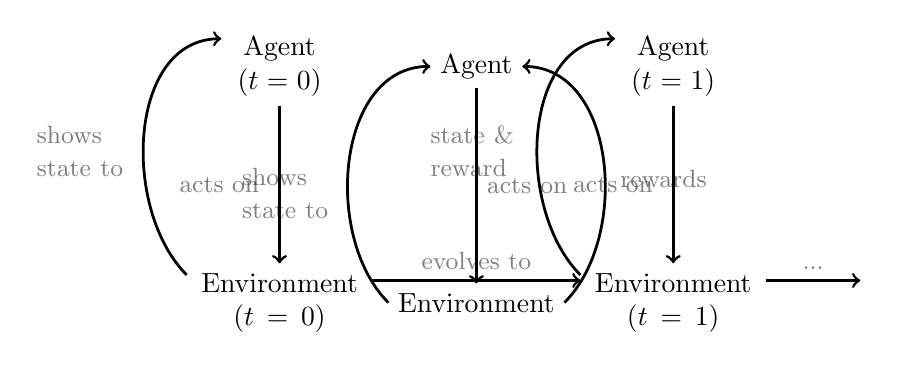
\begin{tikzpicture}[auto]
    \uncover<1-5>{
        \node at (0, 0) (A) {Agent};
    }
    \uncover<2-5> {
        \node at (0, -3) (E) {Environment};
    }
    \uncover<3-5>{
        \path [arrow] (E.west) to [in=180,out=135] node [opacity=0.5, xshift=5pt, yshift=-25pt, text width=40pt] {\small shows state to} (A.west); 
    }
    \uncover<4-5>{
        \path [arrow] (A.south) to  node [opacity=0.5, text width=30pt] {\small acts on} (E.north); 
    }
    \uncover<5>{
        \path [arrow] (E.east) to [in=0,out=45] node [opacity=0.5, xshift=50pt, text width=40pt] {\small rewards} (A.east); 
    }
    \uncover<6-> {
        \node [text width=35pt, align=center] at (-2.5, 0) (A) {Agent (\(t=0\))};
        \node [text width=60pt, align=center] at (-2.5, -3) (E) {Environment (\(t=0\))};
    }
    \uncover<7->{
        \path [arrow] ([yshift=10pt]E.west) to [in=180,out=135] node [opacity=0.5, xshift=5pt, yshift=-20pt, text width=40pt] {\small shows state to} ([yshift=10pt]A.west); 
    }

    \uncover<8->{ 
        \path [arrow] (A.south) to  node [opacity=0.5, xshift=-40pt] {\small acts on} (E.north); 
    }

    \uncover<9->{
        \node [text width=35pt, align=center] at (2.5, 0) (A1) {Agent (\(t=1\))};
        \node [text width=60pt, align=center] at (2.5, -3) (E1) {Environment (\(t=1\))};
    }
    \uncover<10->{
        \path [arrow] ([yshift=8pt]E.east) to node [opacity=0.5] {\small evolves to} ([yshift=8pt]E1.west); 
    }
    \uncover<11->{
        \path [arrow] ([yshift=10pt]E1.west) to [in=180,out=135] node [opacity=0.5, xshift=5pt, yshift=-20pt, text width=40pt] {\small state \& reward} ([yshift=10pt]A1.west); 
    }

    \uncover<12->{ 
        \path [arrow] (A1.south) to  node [opacity=0.5, xshift=-40pt] {\small acts on} (E1.north); 
    }
    \uncover<13>{
        %%\node [text width=35pt, align=center] at (7.5, 0) (A2) {Agent (\(t=2\))};
        \node  at (5, -3) (E2) {};
        \path [arrow] ([yshift=8pt]E1.east) to node [opacity=0.5] {\small ...} ([yshift=8pt]E2.west); 
    }
\end{tikzpicture}
\end{figure}
\end{frame}

\begin{frame}{Agents \& actions}
\begin{columns}
\column{0.5\textwidth}
Agents:
\begin{itemize}
    \item At each time step \(t\), perceives the \textbf{state}, \(s_t\) decides on an \textbf{action}, \(a_t\) from the set of actions available in that state, \(A(s_t)\).
    \item<2-> E.g. press gas, brake, turn wheel left 0.57 radians, press gas + turn right 2.2 radians, shift to 4th gear, ...
\end{itemize}
\column{0.5\textwidth}
    \begin{center}
    \includegraphics[width = \textwidth]{figures/selfdrivingcar.jpg}
    \end{center}
\end{columns}
\end{frame}

\begin{frame}{Environments, states \& transitions}
\begin{columns}
\column{0.5\textwidth}
Environment:
\begin{itemize}
    \item Includes other cars (and also parts of self).
    \item<2-> Is in a state \(s_t\). 
    \item<3-> After the agent takes \(a_t\), evolves to state \(s_{t+1} \in S\) according to the \textbf{transition probabilities}: \(p(s_{t+1} | s_t, a_t)\).
    \item<4-> \textbf{Markov:} transition probabilities depend \emph{only} on \(s_t, a_t\), not history. 
\end{itemize}
\column{0.5\textwidth}
    \begin{center}
    \includegraphics[width = \textwidth]{figures/citystreet.jpg}
    \end{center}
\end{columns}
\note{Sometimes the ``environment'' may include things you intuitively think of as part of the agent, e.g. in the car example the agent would just be the computer, the rest of the car (wheels, etc) would be part of the environment.

So if you're in a state, it doesn't matter how you got to that state} 
\end{frame}


\begin{frame}{Time, \& rewards}
\begin{columns}
\column{0.5\textwidth}
Rewards:
\begin{itemize}
    \item Agent receives a \textbf{reward} \(r_{t+1} \in R\) according to \textbf{reward probabilities}: \(p(r_{t+1} | s_t, a_t, s_{t+1})\). 
    \item<2-> E.g. fare for reaching a destination, penalty for hitting a pedestrian, ...
    \item<3-> \textbf{Return} is the sum of the \textbf{discounted} rewards over time: \(\sum_{t=1}^\infty \gamma^t r_t\) for some \(\gamma \in (0, 1]\).
\end{itemize}
\column{0.5\textwidth}
    \begin{center}
    \includegraphics[width = \textwidth]{figures/money.png}
    \end{center}
\end{columns}
\end{frame}

\begin{frame}[standout]
Questions?
\end{frame}

\section{Learning in MDPs}
\subsection{TD Learning}
\begin{frame}{Chess}
\begin{columns}
\column{0.5\textwidth}
\begin{itemize}
    \item<1-> You're playing chess against Magnus Carlsen. How can you learn?
    \item<2-> It's not supervised, nobody is telling you what the right move was.
    \item<3-> Really the only definite signal you get is the game outcome.
    \item<4-> ... but have you ever had the feeling of ``Oh, f***'' after your opponent makes a move you didn't see?
\end{itemize}
\column{0.5\textwidth}
    \begin{center}
    \includegraphics[width = \textwidth]{figures/chess.jpg}
    \end{center}
\end{columns}
\note{How do you think we do it? Well, sometimes you make a move, and then Magnus moves, and then you're like OH I DIDN'T SEE THAT MY POSITION IS MUCH WORSE THAN I THOUGHT.}
\end{frame}

\begin{frame}{TD Learning (applied to chess)}
\begin{itemize}
    \item<1-> Temporal Difference (TD) learning is a formal framework for learning from surprises. 
    \item<2-> Basic idea: keep a prediction about how things will go, and when you're suprised, revise it. 
    \item<3-> If Magnus surprises you with a forced checkmate, you should definitely revise your understanding of the previous position.
    \item<4-> What exactly are we predicting? 
    \begin{itemize}
        \item<5-> Simple approach: the \emph{value} of every position.
        \item<6-> If we have to re-evaluate a position, we can update our earlier prediction(s).
    \end{itemize}
\end{itemize}
\end{frame}

\begin{frame}{TD Learning (in the brain)}

\begin{center}
\includegraphics[height = 0.9\textheight]{figures/dopamine_TD.png}
\end{center}
\end{frame}

\begin{frame}{TD Learning: Formalism}
\end{frame}

\subsection{Q-learning}


\end{document}
